\section{Background Modeling and Validation}
\label{sec:BackgroundEstimation}

This section describes the strategies for background modeling and validation.
Monte Carlo (MC) simulation is extesively used for model either background and signal, 
in section \ref{sec:SimSamples} a brief description of the simulated sample used is given.

Monte Carlo (MC) Simulation of the background and signal processes is extensively
used that are used to model the backgrounds are described in section~\ref{}.
Monte Carlo simulations of any process are usually prone to systematics
uncertainties due to non-perfect descriptions of pileup effects,
underlying event and detector performance, therefore,
data-driven background esimation method are employed for describe $\Ztautau$ and QCD multijet backgrounds,
described respectively in section~\ref{} and~\ref{}.
%stimate backgrounds from data. In particular for the following cases:
%\begin{itemize}
%  \item[$\bullet$] The $Z \rightarrow \tau\tau \rightarrow ll ~ + ~  4\nu$ is estimated from data using the embedding technique described in Section~\ref{sec:data_mc}.
%  \item[$\bullet$] The multi-jet background is estimated completely from data using the so-called ABCD method.   
%\end{itemize}
Other background processes, such as \ttbar, single top, dibosons, $Z
\rightarrow ll$ + jets (where $l = e,\mu$) and W + jets, are estimated
using MC predictions. Given the particular importance of \ttbar a dedicated study to validate
this background has been made and described in section~\ref{}.

In this section we make use of analysis tools and object definition
(like electrons, jet or muon) described in chapter~\ref{c:detector}. Furthermore
a set corrections is applied to simulated events to take into the non perfect 
description of detector performance and response, full detail on those corrections
is reported in appendix~\ref{}.
Systematic uncertainties on the background model predictions 
are detailed in Section~\ref{sec:Systematics}.

\subsection{Simulated Event Samples}
\label{sec:SimSamples}

%Both the signal and background process modelled by Monte Carlo (MC)
%simulation were produced within the ATLAS MC12a production campaign.
The generators used for the different processes are described below.

Signal production via the gluon fusion process, $gg\rightarrow A/H/h$,
was simulated with POWHEG~\cite{POWHEG} and the associated
$b\bar{b}A/H/h$ production with SHERPA~\cite{SHERPA}.  The
pseudoscalar Higgs boson samples were generated in the mass range from
90~GeV to 400~GeV and 90~GeV to 300~GeV for $ggH$ and $b\bar{b}A$
production, respectively, and at $\tan\beta = 20$. The same kinematics
are assumed for $A/h/H$ Higgs bosons decay products and at other
$\tan\beta$ values. Appropriate reweighting is applied according to the
different cross-sections. The $m_h^{\mathrm{max}}$ MSSM benchmark
scenario~\cite{MSSMmhmax} is assumed.

The production of $W$ and $Z/\gamma^*$ bosons in association with jets
was simulated with the ALPGEN~\cite{Alpgen} generator. 
%This employs
%the MLM matching scheme~\cite{MLM} between the hard process,
%calculated with leading-order matrix elements for up to five jets, and
%the parton shower.  
The $t\bar{t}$ process was generated using the POWHEG generator. The single-top (s-channel, $Wt$)
processes were generated using MC@NLO~\cite{MCatNLO}, while single-top
(t-channel) processes were generated with AcerMC~\cite{AcerMC}.  The
production of diboson~($WW$, $WZ$, $ZZ$) were generated with
HERWIG~\cite{Herwig}.  For all ALPGEN and MC@NLO samples described
above, the parton shower and hadronisation were simulated with HERWIG
and the activity of the underlying event with JIMMY~\cite{JIMMY}.
%The loop-induced $gg\rightarrow WW$ processes were generated using gg2WW~\cite{GG2WW}.  We are not using it Xsec very small
Different parton density functions (PDFs) sets are used depending on
the generator - CTEQ6L1~\cite{CTEQ6} is used by ALPGEN and AcerMC while
CT10~\cite{CT10} is used by SHERPA, POWHEG and MC@NLO. 

The cross-sections of
the MC event samples used in this note are summarised in
Table~\ref{tab:MCxsec}. The $W/Z$+jets and $b\bar{b}A/H/h\rightarrow \tau\tau$ cross sections 
are calculated to NNLO. Those for $\ttbar$ comes from direct cross section measurement \cite{}. The single top and diboson cross sections are calculated at NLO for single top and dibosons. Finally, the direct $gg\rightarrow A/H/h\rightarrow \tau\tau$ signal cross sections 
are calculated at NNLO and NLO for the top loop and the bottom loop and top/bottom loops interference, respectively.

%The values of the steering parameters used for the HERWIG, JIMMY and PYTHIA
%generators are described in Ref.~\cite{ATLASMC09Tune}.
TAUOLA~\cite{TAUOLA} and PHOTOS~\cite{PHOTOS} are used to model the
tau lepton decay and additional photon radiation from charged leptons
in the leading-log approximation, respectively, except for SHERPA
samples.  

All MC event samples were passed through the full simulation
of the ATLAS detector using GEANT4~\cite{Geant4,ATLASSIM} 
%and are reconstructed with the same software version as used for data. 
The effects of the 
simultaneous recording of several events from the
same or neighbouring bunch crossings (pile-up) are considered in the
simulation. 
%Differences between the simulated and actual LHC running
%conditions have been corrected for by re-weighting the simulated
%events according to the distribution of the average number of
%interactions per bunch crossing ($<\mu>$) obtained from the ATLAS
%data.

  
\begin{table}[tp]
\begin{center}
\caption{The cross sections (multiplied by the relevant branching
  ratios~(BR)) used in this note. Signal cross sections are shown for $m_A=150$~GeV and $\tan\beta=20$
\label{tab:MCxsec}
}
\begin{tabular}{cc}
\\
\hline \hline
Process                                                                 & Cross-section~(pb) [$\times$ BR] \\ \hline
$W\rightarrow \ell$+jets ($\ell=e, \mu, \tau$ )                          & 12.22$\times 10^3$ \\
$Z/\gamma^{*}\rightarrow \ell\ell$+jets ($m_{\ell\ell}>60$ GeV)      & 1.15$\times 10^3$ \\
$Z/\gamma^{*}\rightarrow \ell\ell$+jets ($10<m_{\ell\ell}<60$ GeV) & 4.35$\times 10^3$ \\
$t\bar{t}$                                                              & 137.3 \\
Single top $t$-, $s$- and $Wt$-channels                                 & 28.4, 1.8, 22.4 \\
Diboson WW, WZ and ZZ                                                  & 20.6, 6.8, 1.55 \\ \hline
Signal ($m_A=150$~GeV, $\tan\beta=20$, $m_{h}^{max}$ scenario)   &  \\ \hline
$gg\rightarrow A\times$BR$(A\rightarrow\tau\tau)\times$BR$(\tau\tau\rightarrow e\mu+ 4\nu)$                 & $ 16.8 \times 0.118 \times 0.062$ \\
$gg\rightarrow H\times$BR$(H\rightarrow\tau\tau)\times$BR$(\tau\tau\rightarrow e\mu+ 4\nu)$ ($m_H=151$~GeV) & $ 18.4 \times 0.119 \times 0.062$ \\
$gg\rightarrow h\times$BR$(h\rightarrow\tau\tau)\times$BR$(\tau\tau\rightarrow e\mu+ 4\nu)$ ($m_h=129$~GeV) & $ 13.7 \times 0.110 \times 0.062$ \\
$b\bar{b}A\times$BR$(A\rightarrow \tau\tau)\times$BR$(\tau\tau\rightarrow e\mu + 4\nu)$                       & $ 39.4 \times 0.118 \times 0.062$ \\
$b\bar{b}H\times$BR$(H\rightarrow \tau\tau)\times$BR$(\tau\tau\rightarrow e\mu+ 4\nu)$ ($m_H=151$~GeV)       & $ 35.7 \times 0.119 \times 0.062$ \\
$b\bar{b}h\times$BR$(h\rightarrow \tau\tau)\times$BR$(\tau\tau\rightarrow e\mu+ 4\nu)$ ($m_h=129$~GeV)       & $ 4.71 \times 0.110 \times 0.062$ \\
\hline \hline
\end{tabular}
\end{center}
\end{table}


\subsection{Top Quark Pair Production Validation}
\label{sec:top_est}

The background from top quark pair production is estimated using a sample of events from the POWHEG-PYTHIA MC
generator. To validate this MC sample,  a \ttbar rich control region is defined using events passing 
the preselection described in section \ref{sec:eventpresel} with the additional requirement of two b-tagged jets.
%Since this is one of the major backgrounds for this analysis (especially in b-tag category)
%a careful validation of this background model is need, for this purpose a  top quark enriched control region (CR)  
%is defined by adding to the preselection the further requirement of exactly two b-tagged jets in the event. 
Figures~\ref{fig:kinematicsttbar} and~\ref{fig:cutsttbar} show a set of kinematic and analysis selection
variables in this CR, for both data and the MC prediction,  good agreement between data and the background model is found.
%and shows that our top-quark background model describes well the data
Also the prediction of the event yield in this CR is in good agreement with data: an overall
data to background ratio of $0.998 \pm 0.011\mathrm{(stat.)} \pm 0.110 \mathrm{(sys.)}$ is observed. 
The total systematic uncertainty on the ratio is dominated by the uncertainty on the b-tagging efficiency. 
%In addition, this result could be used
%as a measure of $t\bar{t}$ normalisation avoiding systematic uncertainty on the theoretical cross section of
%this process. In this case, however, additional acceptance systematics would need to be evaluated in a dedicated study.
%
%with a dedicated RIVET analysis and uncertainties of the order of the cross section 
%uncertainty are expected, we then drop this possibility considering that wont bring  
%significant improvements.

\begin{figure}[tp]
     \begin{center}

        \subfigure[]{%MMC
            \includegraphics[page=1,width=0.45\textwidth]{figure/bg_estimation/std_plots_twoBtag.pdf}
        }
        \subfigure[]{%ele pT
           \includegraphics[page=6,width=0.45\textwidth]{figure/bg_estimation/std_plots_twoBtag.pdf}
        } 
        \subfigure[]{%Muon pt
            \includegraphics[page=8,width=0.45\textwidth]{figure/bg_estimation/std_plots_twoBtag.pdf}
        }

    \end{center}
    \caption{ Distributions  of a) the MMC mass, b) the transverse momentum of the electron $\pt(e)$ and c) the transverse momentum of the muon $\pt(\mu)$, for both data and MC in the \ttbar control region. The uncertainties on the points for the ratio plot show the statistical uncertainty on the data to background ratio, whereas the yellow band show the total systematic uncertainty on this ratio.} 
   \label{fig:kinematicsttbar}
\end{figure}


\begin{figure}[ht!]
     \begin{center}

        \subfigure[]{
            \label{fig:cuts_a} %DPhi
            \includegraphics[page=12,width=0.45\textwidth]{figure/bg_estimation/std_plots_twoBtag.pdf}
        }
        \subfigure[]{%CosDphi
            \label{fig:cuts_b}
            \includegraphics[page=13,width=0.45\textwidth]{figure/bg_estimation/std_plots_twoBtag.pdf}
        }\\
        \subfigure[]{%Ht
            \label{fig:cuts_c}
            \includegraphics[page=10,width=0.45\textwidth]{figure/bg_estimation/std_plots_twoBtag.pdf}
        }
        \subfigure[]{%Lep+Et
            \label{fig:cuts_d}
            \includegraphics[page=11,width=0.45\textwidth]{figure/bg_estimation/std_plots_twoBtag.pdf}
        }

    \end{center}
    \caption{Distributions of a) $\Delta\phi(e-\mu)$,
      b) $\sum\cos\Delta\phi$, c) \SumLtMET and d) \Ht , for both data and MC in the \ttbar control region. The uncertainty on the points for the ratio plot show the statistical uncertainty on the data to background ratio, whereas the yellow band show the total systematic uncertainty on this ratio.}
   \label{fig:cutsttbar}
\end{figure}


\subsection{Multi-jet Background}
\label{sec:qcd}

The QCD multi-jet background represents an important background, 
especially in the b-veto category, due to its high cross-section and the 
relatively low cut on lepton \pt used in this analysis. This
background is evaluated by a data-driven technique, the so-called ABCD method.
The ABCD method consists of splitting the data sample in four regions: the
 signal region (SR) and three control regions (CR), where the control
regions are mutually orthogonal and designed to be enriched in
multi-jets events. The four regions are defined by using the charge correlation
between the leptons and  isolation selections. With isolation
is intended the sum of the energy deposit in a cone of fixed size around the lepton,
this variable can be defined using calorimetric energy deposition or track momentum 
measurement done by the inner detector.
To obtain regions rich in multi-jet background, the selections on both
the calorimetric and tracking isolation are inverted with respect to the
nominal ones defining anti-isolated leptons, is then
possible to define four regions: opposite sign (OS) or same sign
(SS) with respectively isolated or anti-isolated leptons. Historically
the letters A-D are assigned to this regions for a quicker reference as
defined in Table~\ref{table:qcd}.

\begin{table} [tp]
\centering
\begin{tabular}{c c c }
\hline
Region & Lepton Charge & Lepton Isolation \\ [0.5ex]
\hline
A (signal region) & OS & isolated \\
B & SS & isolated \\
C & OS & anti-isolated \\
D & SS & anti-isolated \\ [1ex]
\hline
\end{tabular}
\caption{QCD background estimation control regions, defined by having leptons with opposite signs (OS) or same signs (SS) and by having the leptons either isolated or anti-isolated.}
\label{table:qcd}
\end{table}

An assumption of the ABCD method is that multi-jet backgrounds
populate the OS and SS events independently of lepton isolation
criteria and hence that the ratio of OS/SS events is uncorrelated 
with the lepton isolation selections. In this case, the number of QCD events in the signal region $A$ 
can be estimated from the yield of multijet events in the control regions $B$, $C$ and $D$, using the equation
\begin{equation} \label{eqn:qcdest}
N_{A}  = N_{B} \times \frac{N_{C}}{N_{D}} =  N_{B} \times \rqcd
\end{equation}
%Here is  assumed that the events in the control regions come solely from QCD multi-jet processes, contamination
%from electroweak (W and Z + jets, dibosons) and top processes
%($t\bar{t}$ and single top production) are  subtracted in each control region 
%using the MC prediction for their event yield.  
To obtain the multijet yields in the data CRs, the contamination
from electroweak (W+jets, Z+jets and dibosons) and top processes
($t\bar{t}$ and single top production) are  subtracted in each control region 
using the MC prediction for their event yield.  Tables~\ref{table:qcd_yield_btag}~and~\ref{table:qcd_yield_bveto}
show the event yield
% in the b-tagged and b-veto categories, respectively,
for each CR throughout the full cut-flows, along with the
predictions of non-QCD multi-jets events which are subtracted.
Signal contamination has been checked in all the three control regions for different 
mass points. For the range of $m_{A}$ and $\mathrm{tan}\beta$ considered in this analysis, the highest signal contamination 
is seen in region B for the mass point $m_{A} = 300$ GeV, where at $\mathrm{tan}\beta = 50$ a contamination 
of 0.2\% is observed. This value is mainly due to b-associated production and,
as it scales with the cross section, for $\mathrm{tan}\beta = 20$ would be an order of magnitude smaller.

Shapes of kinematic distributions for QCD events are taken from the
control region B, even though this region suffers from lower statistics than either region C or D.
This choice is made to avoid a shape bias due to isolation requirements at trigger level.
%the trigger:  an isolated trigger is used 
%for electrons (as described in Section~\ref{sec:eventsel}), where the offline requirement equivalent to this trigger choice is $\ptcone20/\pt <0.1$.
Figure~\ref{fig:BvsD} shows the comparison between the electron \pt~ distributions in isolated 
and anti-isolated events, both for SS control regions. Here high \pt~ electrons are suppressed due to isolation requirement of the the trigger. 
Eventually the trigger isolation requirement could
bias also the ratio OS/SS - this possibility has been checked carefully
in a dedicated study and reported in Appendix \ref{appendix:qcd}.
To a good approximation, such trigger effects cancel out in the ratio
OS/SS, so no systematic is applied to the ratio because of this.

To test the ABCD method predictions an additional control region has been defined with the following selections:
\begin{itemize}
\item \MET $< 20$ GeV
\item \Ht $< 70$ GeV and \SumLtMET$ < 50$ GeV
\item $0 < \mmc < 80$ GeV  	 
\end{itemize}
%{\bf This control region is designed to enhance multi-jet background with respect to \Ztautau.}
Figure~\ref{fig:ABCD_cr} shows the \mmc distribution for this region with and without b-tagging requirements. 
Agreement between data and the background model is found in this control region within statistical and 
detector related systematics uncertainty. 

\begin{figure}[tp]
	\begin{center}
	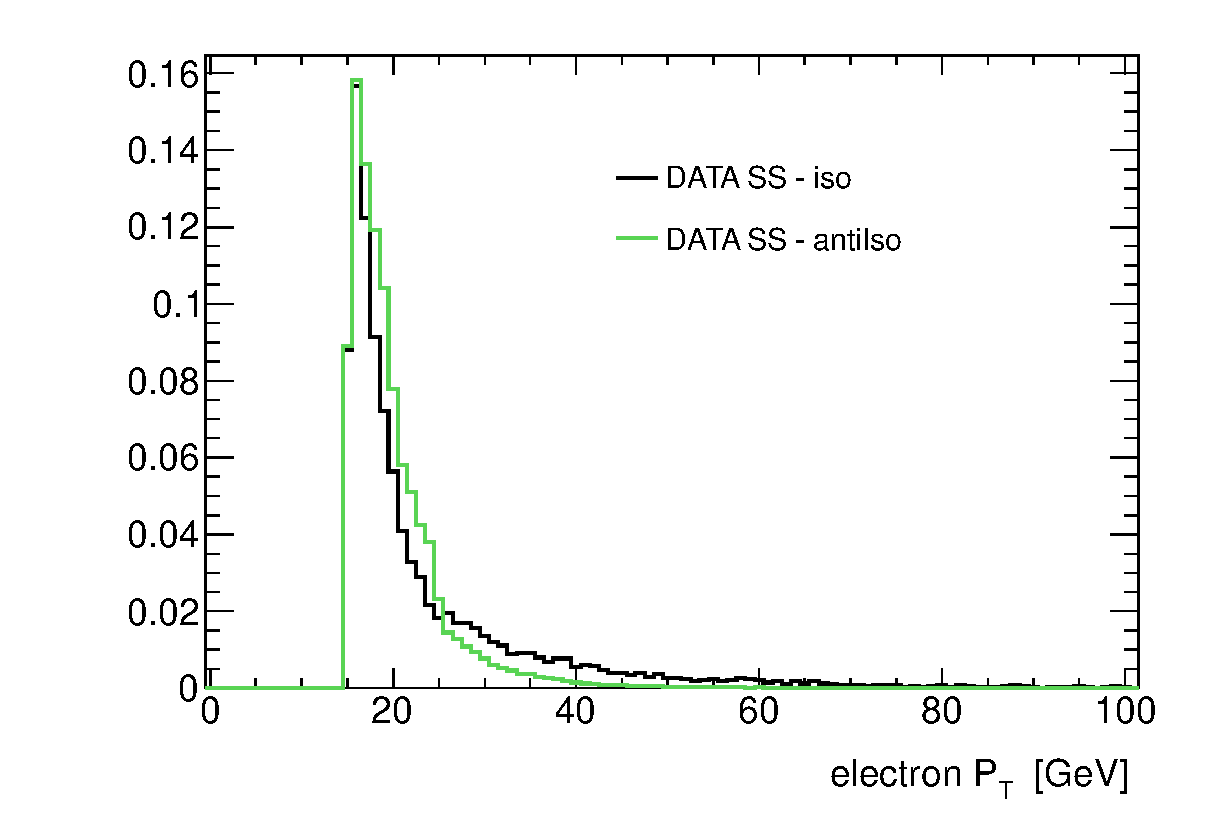
\includegraphics[width=9cm]{figure/ABCD_regionB_Vs_regionD}
	\end{center}
	\caption{Comparison of the electron \pt~distribution in region B and region D, showing the bias due to the trigger. 
	The histograms are normalised to the same area.}
	\label{fig:BvsD}
\end{figure}
%%%%	this table is not that useful

%\begin{table} [p]
%	\caption{Contribution to the different control regions from non-QCD background, after the preselection. }
%	\centering
%	\begin{tabular}{ c c c c c c c}
%%%%%%%%%%%%%%%%%%%%%%%%%%%%%%%%%%%%%%%%%%%%%%%%%%%%%%%%
%\hline
%Region  &  \Ztautau	 & $t\bar{t}$	 & W + jets	 & $Z \rightarrow ll$ + jets & Single Top 	& Dibosons \\ [0.5ex]
%\hline
%  B 	& 341 	$\pm$ 6	&	700$\pm$ 11	&	3398$\pm$ 180	& 830 $\pm$ 58	     &	178$\pm$ 8 		&   612$\pm$ 10  \\
%  C 	& 16 	$\pm$ 2	&	719$\pm$ 12	&	409$\pm$ 50	& 17 $\pm$ 4	     &	103$\pm$ 6		& 13$\pm$ 1 \\
%  D 	& 8	$\pm$ 2	&	539$\pm$ 10	&	49$\pm$	12	& 24$\pm$  7	     &	67$\pm$	 4		& 6$\pm$ 1 \\[1ex]
%\hline
%%%%%%%%%%%%%%%%%%%%%%%%%%%%%%%%%%%%%%%%%%%%%%%%%%%%%%%
%	\end{tabular}
%	\label{table:qcd_mc}
%\end{table}


%%%%%%%%%%%%%%%%%%%%%%%%%%%%%%%%%%%%%%%%%% PUT FINAL NUMBERS!!!!!!!!!!!!!!!! %%%%%%%%%%%%%%%%%%
\begin{table} [p]
	\begin{tabular}[c]{l r c c c c}
%%%%%%%%%%%%%%%%%%%%%%%%%%%%%%%%%%%%%%%%%%%%%%%%%%%%%%
\hline 
\hline 
Selection  &  		& B & C  & D &  \rqcd \\
\hline
Preselection 	&   Data	&6189			&604628			&312901		    &	1.929 $\pm$  	0.004		\\
	        &   non-QCD	&2510 $\pm$  180  	&1090 $\pm$   30  	&730	$\pm$ 35    &				\\
\hline
B-tag	     	&   Data	&419		&44619 			&27257		    &	1.64	$\pm$	0.01	\\
	     	&   non-QCD	&215 $\pm$  10	&310 $\pm$	12	&277 	$\pm$ 13    &				\\
\hline
$\Delta\phi(e-\mu)$  &   Data		&230		&38810 			&23316		    &	1.67	$\pm$	0.01	\\
	     &   non-QCD	&104 $\pm$ 6	&200 $\pm$	10	&175	$\pm$ 7	    &				\\
\hline
$\sum\cos\Delta\phi$ &   Data & 149		&31379 			&18779		    &	1.67	$\pm$	0.02	\\
	     &   non-QCD      & 67 $\pm$ 5	&127 $\pm$	8	&114 $\pm$	6   &				\\
\hline
$\sum H_T$ &   Data	      & 83		& 27781 		&15626		    &	1.78	$\pm$	0.02	\\
	&   non-QCD	      & 23 $\pm$  4	& 25 $\pm$	3	& 22 $\pm$   3	    &				\\ 
\hline
\SumLtMET &   Data	&71		&27735 	&15590		    &	1.78	$\pm$	0.02	\\
	     &   non-QCD	 & 10 $\pm$	3	& 22  $\pm$ 3		&18	$\pm$ 2	    &			\\
\hline
$\mmc > 0.$    &  Data	& 70	& 27634 	& 15522		    			    &	1.78	$\pm$	0.02	\\
	     &   non-QCD	& 9 $\pm$ 3	& 20  $\pm$ 3		&17	$\pm$ 2	    &			\\[1ex]
\hline
\hline
%%%%%%%%%%%%%%%%%%%%%%%%%%%%%%%%%%%%%%%%%%%%%%%%%%%%%%
	\end{tabular}
	  \caption{QCD background estimation as a function of the analysis selections for the b-tagged category. The yields for the different control regions, as well as the scaling factor \rqcd, are reported. The error on the \rqcd is statistical only.}
	\centering
	\label{table:qcd_yield_btag}
\end{table}


\begin{table} [p]
	\begin{tabular}[c]{l r c c c c}
%%%%%%%%%%%%%%%%%%%%%%%%%%%%%%%%%%%%%%%%%%%%%%%%%%%%%%%
\hline
\hline 
Selection  &  		& B & C & D &  \rqcd \\ 
\hline
Preselection 	&   Data	&6189			&604628			&312901		    &	1.929 $\pm$  	0.004		\\
	        &   non-QCD	&2510 $\pm$  180  	&1090 $\pm$   30  	&730	$\pm$ 35    &				\\
\hline
B-veto	     	&   Data	&5673		  & 558217 		& 284847		    &	1.960	$\pm$	0.004	\\
	     	&   non-QCD	&2220	$\pm$ 180 & 710 $\pm$ 30	& 415 $\pm$	30	    &				\\
\hline
$\Delta\phi(e-\mu)i$  &   Data		&4610		&532583 		&271404		    	    &	1.962	$\pm$	0.005	\\
	     &   non-QCD	&1700 $\pm$170	&580 $\pm$	30	& 345 $\pm$	30	    &				\\
\hline
$\sum\cos\Delta\phi$ &   Data& 3417	&486747 		& 247712	   		    &	1.965	$\pm$	0.005 	\\
	     &   non-QCD     & 1120  $\pm$ 100	& 370 $\pm$ 	20		& 230 $\pm$	20  &				\\
\hline
$\mmc > 0.$    &  Data		& 3177		& 479967 		& 244276	    	    &	1.965	$\pm$	0.005	\\
	     &   non-QCD	& 1000 $\pm$ 100	& 300  $\pm$ 17		&190	$\pm$ 20    &			\\[1ex]
\hline
\hline
%%%%%%%%%%%%%%%%%%%%%%%%%%%%%%%%%%%%%%%%%%%%%%%%%%%%%%%
	\end{tabular}
	\caption{QCD background estimation as a function of the analysis selections for b-veto category. The yields for the different control regions, as well as the scaling factor \rqcd, are reported. The error on the \rqcd is statistical only.}
	\centering
	\label{table:qcd_yield_bveto}
\end{table}



\begin{figure}[tp]
	\begin{center}
	     
	\subfigure[]{
		\includegraphics[page=1,width=0.49\textwidth]{figure/QCD/qcd_CR_emb.pdf}
	        }
	\subfigure[]{
  	\includegraphics[page=5, width=0.49\textwidth]{figure/QCD/qcd_CR_emb.pdf}
	}
	
	\end{center}
	\caption{\mmc distribution for QCD cross check regions defined in section \ref{sec:qcd} (a) and for the same CR when in addition one b-tagged jet is required (b). }
	\label{fig:ABCD_cr}
\end{figure}


Systematic uncertainties are assigned on the scaling factor \rqcd and on the shape of
the discriminating variable \mmc to take into account any correlation between isolation and charge 
of the leptons, details on the systematic uncertainty evaluation are addressed in Section~\ref{sec:Systematics}.





\subsection{$Z \rightarrow \tau\tau$ + Jets Background: Embedding Technique}
The background from \Ztautau decays is the major background to this analysis, a good uderstanding 
of it is then extremely important.
 Unfortunately, for a light Higgs boson, it is impossible to completely separate \Ztautau decays 
from the signal and signal free data control region cannot be defined.
However, thanks to the small Higgs coupling to muons, \Zmumu decays provide a good starting point to 
model \Ztautau events in a data-driven way. An hybrid Data-MC sample, known as "Embedding" is used to model the \Ztautau background: 
$\Zmumu$ candidates are selected in data, then the two muons from the $Z$ decay are substituted with the decay 
products from simulated taus, this means that also the energy in a cone around the muon is subtracted
and substituted with the one from tau decay, those taus have the same kinematics as the original muons. 
Further details may be found in \cite{Embedding, SMold}.

%The selection of the \Zmumu input data requires exactly two combined, opposite charged
%muons, where the leading muon has a transverse momentum $\pt > 20 \GeV$ and 
%the subleading muon $\pt > 15\GeV$. Both muons are requited to lie within $|\eta|<2.5$ and to be isolated with 
%$\ptcone 20/\pt<0.2$ (see Section~\ref{sec:presel}). Additionally 
%the invariant mass of the two muons is required to be in the range $M_{\mu\mu} > 40$ GeV.
%Once the muon pair events are selected, all tracks and calorimeter cells associated to the muons are 
%removed from the \Zmumu data event. Finally, the calorimeter cell energy and tracks from the simulated tau decays
%are added to the data event and the event is re-reconstructed.

%A set of corrections are applied to correct for the muon trigger efficiency, the muon reconstruction efficiency and other additional effects
%related to the original \Zmumu events. Finally, as the trigger is not emulated in the embedding sample, 
%an additional correction is applied to emulate the electron and muon trigger efficiencies in the final \Ztautau embedded events. 
%For a full description of the corrections and validation see \cite{SMnew}.

%The Embedding technique, which uses \Zmumu decays to 
%model \Ztautau events in a data-driven way, is described in Section~\ref{sec:data_mc}. 
There is no simulation of the trigger in the embedding samples, the event yield
is normalised to ALPGEN \Ztautau at preselection stage. Furthermore a set of corrections, as described in \cite{SMnew}, are
applied to unfold from the trigger and muon reconstruction efficiency of 
the original \Zmumu events, then trigger and reconstruction efficiency for muon and electron is emulated 
by the use of event weight.

The Embedding technique has been validated in several studies, detailed in~\cite{Embedding, SMnew}, which show a good description of 
data and \Ztautau MC by Embedding. In the context of this analysis, 
figures~\ref{fig:emb_vs_alp1} and \ref{fig:emb_vs_alp} show comparisons of various kinematic variables between
data, embedding and ALPGEN \Ztautau events at preselection. No significant deviation is seen 
between the \mmc distribution of the embedding and ALPGEN samples. 
However other relevant variables for this analysis, such as the \MET 
and the number of b-jets, are slightly better described by embedding. Additional plots are 
reported in appendix~\ref{appendix:additionalEmb}.

\begin{figure}[tp]
     \begin{center}

            \includegraphics[page=1, width=0.6\textwidth]{figure/bg_estimation/std_plots_emb.pdf}
\end{center}
    \caption{Comparison between the embedded \Ztautau and ALPGEN for $\mmc$ distributions.}
   \label{fig:emb_vs_alp1}
\end{figure}


\begin{figure}[tp]
     \begin{center}

           \includegraphics[page=2, width=0.6\textwidth]{figure/bg_estimation/std_plots_emb.pdf}
            \includegraphics[page=3, width=0.6\textwidth]{figure/bg_estimation/std_plots_emb.pdf}

    \end{center}
    \caption{Comparison between embedded \Ztautau and ALPGEN for $\MET$ and the number of b-tagged jets distributions.
	Data are superimposed, with the contribution of non-\Ztautau are subtracted.}
   \label{fig:emb_vs_alp}
\end{figure}


%plot comparing embedding and ALPGEN Et miss and b-tagging, data -MC not Ztautau and compare data alp and emb.

The Embedding sample is based on selecting \Zmumu candidates in data, the selections assure a rather 
pure \Zmumu sample, however further selections used in this analysis, for example the b-tagging requirements, 
could enhance the contamination fraction from other processes in the embedding sample. Hence dedicated studies have been
made to estimate the $t\bar{t}$ and QCD multi-jet contamination in the embedding sample.
The \ttbar~ contamination is estimated by evaluating the embedding sample yield in a two b-tag control region,
as described in Section~\ref{sec:top_est}. These events are assumed to be solely from $t\bar{t}$
and their yield in the signal region is extrapolated using POWHEG-PYTHIA $t\bar{t}$ simulation sample.
Table~\ref{table:emb_cont_tt} shows a summary for the top contamination in embedding and this contamination is hence taken to be negligible. The multi-jet contamination can be estimated starting 
from the embedding yield of opposite sign anti-isolated events (region C).
%one should not use SS regions because embedding already requires leptons to be OS, then would be biased
Assuming all events in this CR as QCD multi-jet events, the contamination in the SR 
can be estimated using the ABCD method (see Section\ref{sec:qcd}). The \rqcd factor 
used in this case is evaluated using a mu-mu final state CR with the same kinematics selections
used in the definition of the embedding sample. Table~\ref{table:emb_cont_qcd}
shows the estimated contamination of QCD multi-jet in embedding. 
We  consider contamination effects negligible.


\begin{table} [tp]
\centering
\begin{tabular}{c c c c c}
\hline
\hline
 & Embedding	& Transfer	& Estimated	& Contamination \\
 & yield in CR	& factor	& events in SR	&	\\		 [0.5ex]
\hline
b-tag & $84 \pm 9$  & $(2.6 \pm 0.1) \times 10^{-2}$ &  $2.2 \pm 0.2$&  0.5 \% \\
b-veto & $84 \pm 9$ & $(1.74 \pm 0.02) \times 10^{-1}$ & $15 \pm 2$ & 0.03 \% \\[1ex]
\hline
\end{tabular}
\caption{Evaluating embedding $t\bar{t}$ contamination using a two b-tag CR. The transfer factor is the
multiplicative factor that allows to estimate events in SR from the CR. }
\label{table:emb_cont_tt}
\end{table}

\begin{table} [tp]
\centering
\begin{tabular}{c c c c c}
\hline
\hline
 & Embedding	& Transfer	& Estimated	& Contamination \\
 & yield in CR	& factor	& events in SR	&	\\		 [0.5ex]
\hline
B-tag  & $12 \pm 3$ & $ (7 \pm 1) \times 10^{-3}$ &  $(8.4 \pm 0.3) \times 10^{-2}$ &  0.03 \% \\
B-veto & $390 \pm 20$ & $(2.5 \pm 0.1) \times 10^{-2}$ & $10.0 \pm 0.5$ & 0.02 \% \\[1ex]
\hline
\end{tabular}
\caption{Evaluating embedding contamination due to QCD multi-jet using ABCD method, 
the CR here is with OS anti-isolated events (region C). The transfer factor is the
multiplicative factor that allows to estimate events in SR from the CR, in this case is $N_{B} / N_{D}$
and is evaluated using mu-mu final state with the same kinematic selection used in the 
definition of the embedding sample. }
\label{table:emb_cont_qcd}
\end{table}



